\documentclass[xcolor={table}]{beamer}
\usepackage{fleqn}
\usepackage{graphicx}
\usepackage{coordsys} %for \numbline commander

%Setup appearance:
\usetheme{Darmstadt}
\usefonttheme[onlylarge]{structurebold}
\setbeamerfont*{frametitle}{size=\normalsize,series=\bfseries}
\setbeamertemplate{navigation symbols}{}
\setbeamertemplate{bibliography item}{[\theenumiv]}

% Standard packages
\usepackage[english]{babel}
\usepackage[latin1]{inputenc}
\usepackage{times}
\usepackage[T1]{fontenc}
\usepackage{multirow}
\usepackage{subfigure}
\usepackage{pbox}
\usepackage{arydshln}
\usepackage{pifont}
\usepackage{cancel}
\usepackage{rotating} % for sideways headings

% Source Code packages
\usepackage{algorithm2e}
\usepackage{algorithmic}

\DeclareSymbolFont{extraup}{U}{zavm}{m}{n}
\DeclareMathSymbol{\varclub}{\mathalpha}{extraup}{84}
\DeclareMathSymbol{\varspade}{\mathalpha}{extraup}{85}
\DeclareMathSymbol{\varheart}{\mathalpha}{extraup}{86}
\DeclareMathSymbol{\vardiamond}{\mathalpha}{extraup}{87}

%%% This section command that adds a big page with section dividers
\usepackage{xifthen}% provides \isempty test
\newcommand{\SectionSlide}[2][]{
	\ifthenelse{\isempty{#1}}
		{\section{#2}\begin{frame} \begin{center}\begin{huge}#2\end{huge}\end{center}\end{frame}}
		{\section[#1]{#2}\begin{frame} \begin{center}\begin{huge}#2\end{huge}\end{center}\end{frame}}
}
%Extends the section slide to to include a shortened section title for the navigation bar as a second parameter
\newcommand{\SectionSlideShortHeader}[3][]{
	\ifthenelse{\isempty{#1}}
		{\section[#3]{#2}\begin{frame} \begin{center}\begin{huge}#2\end{huge}\end{center}\end{frame}}
		{\section[#1]{#2}\begin{frame} \begin{center}\begin{huge}#3\end{huge}\end{center}\end{frame}}
}

\newcommand{\refer}[1]{\footnote{#1}}
\newcommand{\GW}{\text{\textit{Guess-Who~}}}
\newcommand{\keyword}[1]{\alert{\textbf{#1}}\index{#1}}
\newcommand{\firstkeyword}[1]{\textbf{#1}\index{#1}}
\newcommand{\indexkeyword}[1]{\alert{\textbf{#1}\index{#1}}}
\newcommand{\featN}[1]{\textsc{#1}}
\newcommand{\featL}[1]{\textit{'#1'}}
 \newcommand{\ourRef}[1]{\ref{#1} $^{\text{\tiny[\pageref{#1}]}}$}
 \newcommand{\ourEqRef}[1]{\eqref{#1}$^{\text{\tiny[\pageref{#1}]}}$}
  
\DeclareMathOperator*{\argmax}{argmax}
\DeclareMathOperator*{\argmin}{argmin}



\title{Evaluation\\Sections $9.1, 9.2, 9.3$}
	\author{John D. Kelleher and Brian Mac Namee and Aoife D'Arcy}
	\institute{}
	\date{}

\begin{document}
\begin{frame}
	\titlepage
\end{frame}
\begin{frame}
	 \tableofcontents
\end{frame}


\section{Big Idea}

\begin{frame}
	\begin{itemize}
		\item The most important part of the design of an evaluation experiment for a predictive model is ensuring that the data used to evaluate the model is not the same as the data used to train the model.
	\end{itemize}
\end{frame}

\section{Fundamentals}

\begin{frame}
\begin{itemize}
	\item The purpose of evaluation is threefold:
	\begin{enumerate}
		\item to determine which model is the most suitable for a task
		\item to estimate how the model will perform
		\item to convince users that the model will meet their needs
	\end{enumerate}
\end{itemize}
\end{frame}

\SectionSlide{Standard Approach: Measuring Misclassification Rate on a Hold-out Test Set}



 \begin{frame} 
\begin{figure}[htb]
       \begin{centering}
			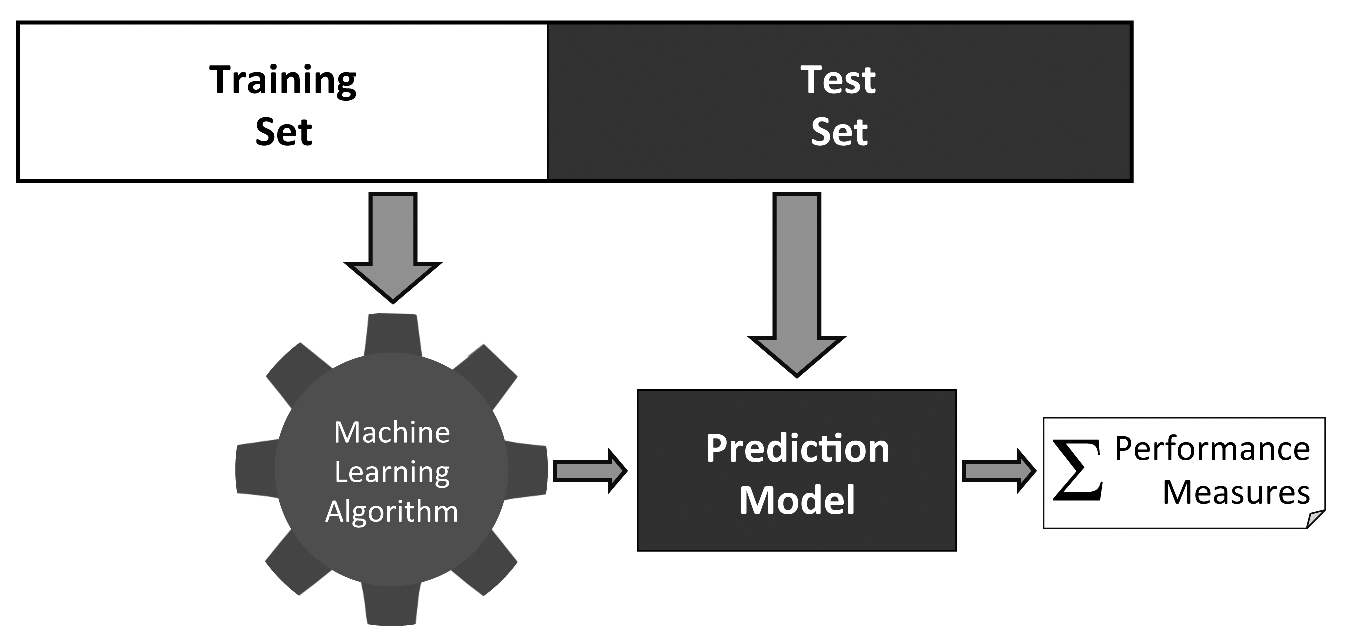
\includegraphics[width=0.75\textwidth]{images/EvaluationProcessesHoldOut2_BW.pdf}
       \caption{The process of building and evaluating a model using a \indexkeyword{hold-out test set}.}
       \label{fig:holdoutTestSetProcess}
       \end{centering}
\end{figure}
\end{frame} 

 \begin{frame} 
\begin{table}[!tb]
\caption{A sample test set with model predictions.}
\label{tab:samplePredictionExample}
\centering
\begin{scriptsize}
\begin{tabular}{cc}
		\hline
			\begin{minipage}{0.45\textwidth}
					\begin{tabular}{ c c c c}
\featN{ID}	 & Target	& Pred. & Outcome\\
\hline
1	&	spam	&	ham	&	FN	\\ 
2	&	spam	&	ham	&	FN	\\
3	&	ham	&	ham	&	TN	\\
4	&	spam	&	spam	&	TP	\\
5	&	ham	&	ham	&	TN	\\
6	&	spam	&	spam	&	TP	\\
7	&	ham	&	ham	&	TN	\\
8	&	spam	&	spam	&	TP	\\
9	&	spam	&	spam	&	TP	\\
10	&	spam	&	spam	&	TP	\\
\hline 
\end{tabular}
			\end{minipage}
			&
			\begin{minipage}{0.45\textwidth}
									\begin{tabular}{ c c c c}
\featN{ID}	 & Target	& Pred. & Outcome\\
\hline
11	&	ham	&	ham	&	TN	\\
12	&	spam	&	ham	&	FN	\\
13	&	ham	&	ham	&	TN	\\
14	&	ham	&	ham	&	TN	\\
15	&	ham	&	ham	&	TN	\\
16	&	ham	&	ham	&	TN	\\
17	&	ham	&	spam	&	FP	\\
18	&	spam	&	spam	&	TP	\\
19	&	ham	&	ham	&	TN	\\
20	&	ham	&	spam	&	FP	\\
\hline 
\end{tabular}
			\end{minipage}\\
\end{tabular}
\end{scriptsize}
\end{table}
\end{frame} 


 \begin{frame} 
\begin{alignat}{2}
\text{misclassification~rate} & = \frac{\text{number incorrect predictions}}{\text{total predictions}}
\end{alignat}
\pause
 \begin{alignat*}{2}
\text{misclassification~rate} & = \frac{\left(2 + 3\right)}{\left(6 + 9 + 2 + 3\right)} & \,= 0.25
\end{alignat*}
\end{frame} 

\begin{frame}
	\begin{itemize}
		\item For binary prediction problems there are 4 possible outcomes:
		\begin{enumerate}
			\item True Positive (TP)
			\item True Negative (TN)
			\item False Positive (FP)
			\item False Negative (FN)
		\end{enumerate}
	\end{itemize}
\end{frame}

 \begin{frame} 
\begin{table}
\caption{The structure of a confusion matrix.}
\label{tab:confusionMatrixStucture}
\centering
\begin{footnotesize}
\begin{tabular}{c >{\bfseries}r @{\hspace{0.7em}} | c @{\hspace{0.4em}} c @{\hspace{0.7em}}}
    & &  \multicolumn{2}{c}{\bfseries Prediction} \\
  & & \bfseries positive & \bfseries negative  \\
  \hline
  \multirow{2}{*}{\parbox{1.1cm}{\bfseries\raggedleft Target}}  & positive & $TP$	&	$FN$ \\
  & negative & $FP$	&	$TN$
\end{tabular}
\end{footnotesize}
\end{table}
\end{frame} 

 \begin{frame} 
\begin{table}
\caption{A confusion matrix for the set of predictions shown in Table \ourRef{tab:samplePredictionExample}.}
\label{tab:confusionMatrixExample}
\centering
\begin{footnotesize}
\begin{tabular}{c >{\bfseries}r @{\hspace{0.7em}} | c @{\hspace{0.4em}} c @{\hspace{0.7em}}}
    & &  \multicolumn{2}{c}{\bfseries Prediction} \\
  & & \bfseries \featL{spam} & \bfseries \featL{ham} \\
  \hline
  \multirow{2}{*}{\parbox{1.1cm}{\bfseries\raggedleft Target}}  & \featL{spam} & $6$	&	$3$ \\
  & \featL{ham} & $2$	&	$9$ 
\end{tabular}
\end{footnotesize}
\end{table}
\end{frame} 

 \begin{frame} 
\begin{alignat}{2}
\text{misclassification~accuracy} & = \frac{\left(FP + FN\right)}{\left(TP + TN + FP + FN\right)}
\end{alignat}
\pause
\begin{alignat*}{2}
\text{misclassification~accuracy} & = \frac{\left(2 + 3\right)}{\left(6 + 9 + 2 + 3\right)} & \,= 0.25
\end{alignat*}
\end{frame} 

 \begin{frame} 
\begin{alignat}{2}
\text{classification~accuracy} & = \frac{\left(TP + TN\right)}{\left(TP + TN + FP + FN\right)}
\end{alignat}
\pause
\begin{alignat*}{2}
\text{classification~accuracy} & = \frac{\left(6 + 9\right)}{\left(6 + 9 + 2 + 3\right)} & \,= 0.75
\end{alignat*}
\end{frame} 

\SectionSlide{Summary}

\begin{frame}
	\tableofcontents
\end{frame}

\end{document}
